
\documentclass[11pt]{article}
 
\usepackage{amstex}
\usepackage[dvips]{epsfig}

\def\proclaim#1{{\bf #1} \it}
\def\endproclaim{\normalfont}

\def\tW{\tilde W}
\def\Aut{\text{Aut}}
\def\tr{{\text{tr}}}
\def\ell{{\text{ell}}}
\def\Ad{\text{Ad}}
\def\u{\bold u}
\def\m{\frak m}
\def\O{{\cal O}}
\def\tA{\tilde A}
\def\qdet{\text{qdet}}
\def\k{\kappa}
\def\RR{\Bbb R}
\def\be{\bold e}
\def\bR{\overline{R}}
\def\tR{\tilde{{\cal R}}}
\def\hY{\hat Y}
\def\tDY{\widetilde{DY}(\g)}
\def\R{\Bbb R}
\def\h1{\hat{\bold 1}}
\def\hV{\hat V}
\def\deg{\text{deg}}
\def\hz{\hat \z}
\def\hV{\hat V}
\def\Uz{U_h(\g_\z)}
\def\Uzi{U_h(\g_{\z,\infty})}
\def\Uhz{U_h(\g_{\hz_i})}
\def\Uhzi{U_h(\g_{\hz_i,\infty})}
\def\tUz{U_h(\tg_\z)}
\def\tUzi{U_h(\tg_{\z,\infty})}
\def\tUhz{U_h(\tg_{\hz_i})}
\def\tUhzi{U_h(\tg_{\hz_i,\infty})}
\def\hUz{U_h(\hg_\z)}
\def\hUzi{U_h(\hg_{\z,\infty})}
\def\Uoz{U_h(\g^0_\z)}
\def\Uozi{U_h(\g^0_{\z,\infty})}
\def\Uohz{U_h(\g^0_{\hz_i})}
\def\Uohzi{U_h(\g^0_{\hz_i,\infty})}
\def\tUoz{U_h(\tg^0_\z)}
\def\tUozi{U_h(\tg^0_{\z,\infty})}
\def\tUohz{U_h(\tg^0_{\hz_i})}
\def\tUohzi{U_h(\tg^0_{\hz_i,\infty})}
\def\hUoz{U_h(\hg^0_\z)}
\def\hUozi{U_h(\hg^0_{\z,\infty})}
\def\hg{\hat\g}
\def\tg{\tilde\g}
\def\Ind{\text{Ind}}
\def\pF{F^{\prime}}
\def\hR{\hat R}
\def\tF{\tilde F}
\def\tg{\tilde \g}
\def\tG{\tilde G}
\def\hF{\hat F}
\def\bg{\overline{\g}}
\def\bG{\overline{G}}
\def\Spec{\text{Spec}}
\def\tlo{\hat\otimes}
\def\hgr{\hat Gr}
\def\tio{\tilde\otimes}
\def\ho{\hat\otimes}
\def\ad{\text{ad}}
\def\Hom{\text{Hom}}
\def\hh{\hat\h}
\def\a{\frak a}
\def\t{\hat t}
\def\Ua{U_q(\tilde\g)}
\def\U2{{\Ua}_2}
\def\g{\frak g}
\def\n{\frak n}
\def\hh{\frak h}
\def\sltwo{\frak s\frak l _2 }
\def\Z{\Bbb Z}
\def\C{\Bbb C}
\def\d{\partial}
\def\i{\text{i}}
\def\ghat{\hat\frak g}
\def\gtwisted{\hat{\frak g}_{\gamma}}
\def\gtilde{\tilde{\frak g}_{\gamma}}
\def\Tr{\text{\rm Tr}}
\def\l{\lambda}
\def\I{I_{\l,\nu,-g}(V)}
\def\z{\bold z}
\def\Id{\text{Id}}
\def\<{\langle}
\def\>{\rangle}
\def\o{\otimes}
\def\e{\varepsilon}
\def\RE{\text{Re}}
\def\Ug{U_q({\frak g})}
\def\Id{\text{Id}}
\def\End{\text{End}}
\def\gg{\tilde\g}
\def\b{\frak b}
\def\S{{\cal S}}
\def\L{\Lambda}
 



\title {Lecture 2: Perturbative renormalization (continued)}
\author {Edward Witten}
 
\begin{document}
  
\begin{center}
{\LARGE\bfseries{Lecture 2: Perturbative renormalization (continued)} }\\
\vskip 1em%
{\Large Edward Witten}\footnote{\tt 
Notes by Pasha Etingof and David Kazhdan, TeXnical editing Misha Verbitsky} 
      \vskip 1.5em%
    {\large October 1996} \\ 
\end{center}
 
\subsection*{2.1. Renormalizability of quantum field theories.}
Last week we considered the $\phi^3$ theory and found that its 
renormalizability (i.e. how many graphs are divergent,
and how badly divergent they are)
depends on whether $n<6$, $n=6$, or $n>6$. Now we will see how to find
that the critical value of $n$ in the $\phi^3$ theory is 6 without 
considering any graphs at all. 

In order to find the critical value of $n$,
we will define and compute the homogeneity degree of all terms
in the Lagrangian. 
We recall that the Lagrangian is
$$
\int(\frac{1}{2}(\nabla\phi)^2+\frac{1}{2}m^2\phi^2+\frac{g}{3!}\phi^3)d^nx,
\leqno{(2.1)}
$$
(we are considering the Euclidean theory; in the Minkowski version,
the story is the same).
Consider the dilation $x\to t^{-1}x$, $t\in\R$, $x\in V$.
Under this transformation $d^nx\to t^{-n}d^nx$, $\nabla\to 
t\nabla$.  
If we want the integral (2.1) to be invariant under this dilation, 
we must impose the following three transformation laws:
$(\nabla \phi)^2\to t^n(\nabla\phi)^2$, $m^2\phi^2\to t^nm^2\phi^2$, 
$g\phi^3\to t^ng\phi^3$. From the first law we get 
$\phi\to t^{\frac{n-2}{2}}\phi$, from the second
$m\to tm$, and from the third $g\to t^{\frac{6-n}{2}}g$. 
In the future we will write these scaling laws like this:
$$
[x]=-1, [d^nx]=-n,[\nabla]=1,[\phi]=\frac{n-2}{2},[m]=1,[g]=\frac{6-n}{2}.
\leqno{(2.2)}
$$
In other words, any homogeneous quantity 
$a$ scales as $a\to t^{[a]}a$ under the 
dilation, and the number $[a]$ is called the dimension of $a$.

{\bf Remark.} It is not difficult to define the notion of dimension completely 
formally (using the tensor calculus on the tangent bundle of $V$), but
it is more illuminating to illustrate it on examples.
 
We see that the number $6$ appears in the scaling law for $g$. 
More precisely, 
we see that the behavior of the $\phi^3$ theory is determined by 
whether $[g]$ is positive, zero, or negative. 
Namely, we have three cases.

1. $[g]>0$ ($n<6$): 
there is a finite number of superficially divergent graphs 
(by graphs we always mean connected graphs).

2. $[g]=0$ ($n=6$): the number of superficially divergent graphs is infinite,
but $div(\Gamma)$ is bounded from above.

3. $[g]>0$ ($n>6$): there are infinitely many graphs with 
any number of external vertices and arbitrarily high 
$div(\Gamma)$. 

Now we will explain why
this method works, and
prove that it can be used to compute the critical value of the dimension
of the spacetime in a general 
field theory.
In general, we can consider the following setup. 
Suppose we have a quantum field theory with fields $\phi_1,...,\phi_N$, and
the Lagrangian 
$$
{{\cal L}}=\int (\sum_iQ_i(\phi_i)+\sum_k g_kI_k(\phi_1,...,\phi_N))d^nx,
\leqno{(2.3)}
$$ 
where $Q_i$ is a free (quadratic) part, 
and $I_k$ are interaction 
(coupling) terms (differential monomials in fields, cubic and higher). 
Each interaction
term comes with a small parameter
$g_k$, which is called the coupling constant. 

\proclaim{Definition} An interaction $I_k$ is called subcritical
if $[g_k]>0$, and critical if $[g_k]=0$.
A field theory is called superrenormalizable if all interaction terms
in the Lagrangian are subcritical, and is called renormalizable,
or critical, if all interaction terms are critical or subcritical, but not all of them are subcritical.
Otherwise, the theory is called non-renormalizable.
\endproclaim

For example, the $\phi^3$ theory is superrenormalizable 
for $n<6$, renormalizable for $n=6$, and non-renormalizable for
$n>6$. 

We will assume that our theory is a perturbation of a free theory, 
(for the definition of a free theory, see Kazhdan's lectures). 
In a free theory, one can easily see that the dimension
of bosonic fields is $\frac{n-2}{2}$, and of fermionic fields
is $\frac{n-1}{2}$. Since dimensions of fields are determined from the
quadratic part of the Lagrangian, these dimensions will be the same in the
perturbed (classical) theory as well.
 
We will also assume that $n\ge 2$
(In the quantum mechanical case $n=1$ renormalization 
theory is not necessary).
Then $[\phi_i]\ge 0$.

\proclaim{Theorem 2.1} (i) If a theory is superrenormalizable,
there is a finite number of superficially divergent graphs
in its Feynman diagram expansion. 

(ii) If a theory is renormalizable then
the number of superficially divergent graphs is infinite,
but $div(\Gamma)$ is bounded from above. 

(iii). If a theory is non-renormalizable
then there are infinitely many graphs with any number of external 
vertices and arbitrarily high 
$div(\Gamma)$. 
\endproclaim

{\bf Proof} Let $\Gamma$ be a graph in the Feynman 
diagram expansion of our theory. Types of internal vertices of such a graph
correspond to interaction terms in the Lagrangian, and types of its external
vertices and
edges correspond to fields $\phi_i$. Let $e_i$ be the number of external
vertices of type $\phi_i$, and $v_k$ be the number of internal vertices 
of type $I_k$.
Then it is easy to show that
$$
div(\Gamma)=n-\sum_ie_i[\phi_i]-\sum_kv_k[g_k].\leqno{(2.4)}
$$
Statements (i)-(iii) of the theorem follows immediately from (2.4).
%\enddemo

\proclaim{Definition} A theory of the form (2.3) is called 
classically scale invariant if
the n-form under the integral in the Lagrangian is invariant under dilations. 
\endproclaim

For example, the theory of a free scalar field is scale invariant iff it is 
massless. 

It is clear that a massless theory is scale invariant if and only if 
it is purely critical, i.e. $[g_k]=0$ for all $k$. 

{\bf Remark.} Scale invariant theories are always conformal.
Indeed, the Lagrangian is 
always written naturally in terms of the metric on the 
spacetime, and depends only on the fields and their first derivatives. 
This implies that a scale invariant Lagrangian has to be 
invariant under conformal changes of metric.
 
\subsection*{2.2. Critical dimensions of some field theories.}

Now we will compute the critical dimension for several 
important field theories.

{\bf Example 1. Sigma-models.}

Let $M$ be a Riemannian manifold. The Lagrangian of the sigma-model
on $\R^n$ with the target space $M$ is 
$$
{\cal L}(\phi)=\int d^nx g_{ij}(\phi)\nabla\phi^i\cdot\nabla\phi^j.\leqno{(2.5)}
$$
Since this theory is conformal in two dimensions, $2$ must be the critical
dimension. Let us show by a direct computation
that this theory is not renormalizable for $n>2$. 

Let $\phi_i$ be coordinates on $M$ near some point. 
If the metric $g_{ij}$ is constant in these coordinates, the theory is free. 
Consider a nonconstant metric of the form
$$
g_{ij}(\phi)=\delta_{ij}+a_{ijk}\phi^k+r_{ijkl}\phi^k\phi^l+...\leqno{(2.6)}
$$
(If we chose normal coordinates, we could get rid of $a$, but not of $r$,
as $r$ in normal coordinates is the Riemann curvature tensor).
Substituting this into the Lagrangian, we find 
that $[r]=2-n$. This shows that sigma-model is not renormalizable 
beyond $n\ge 2$, unless the metric is flat. 

{\bf Example 2. Gravity.}

In the theory of gravity 
the spacetime is the space $\R^n$ with a metric of the form
$g_{ij}=\delta_{ij}+h_{ij}\sqrt{G}$, where $G$ is the Newton's constant
(for us, it is just a formal parameter). The Lagrangian of the theory is
$$
{\cal L}(g)=\frac{1}{G}\int R(g)d^nx,\leqno{(2.7)}
$$
where $R(g)$ is the scalar curvature of the metric. 
In terms of $h$, this Lagrangian can be rewritten as
$$
{\cal L}=\int d^nx ((\nabla h)^2+\sqrt{G}h(\nabla h)^2+...),\leqno{(2.8)}
$$
so we get $[h]=\frac{n-2}{2}$, $[G]=2-n$. Thus, as in the previous 
example, the theory is non-renormalizable for $n>2$ and critical for $n=2$. 

{\bf Remark.} Here $h(\nabla h)^2$ stands for an expression which is 
linear in $h$ and quadratic in $\nabla h$. It is easy to compute what it is
exactly, but it does not matter to us, since we are only interested
in the dimension. So we will use such sloppy notation.
  
{\bf Example 3. Gauge theory.} 

In gauge theory fields are conections in a fixed principal
$G$-bundle on the space $\R^n$, where $G$ is a compact Lie group.
The Lagrangian has the form 
$$
{\cal L}(\tilde A)=\frac{1}{e^2}\int \Tr(F_{\tilde A}\wedge 
*F_{\tilde A}),\leqno{(2.9)}
$$
where $F_{\tilde A}$ is the curvature of the connection $\tilde A$, 
and $\Tr$ is an invariant nondegenerate bilinear form on the Lie algebra $\g$
of $G$. 

In the computation of dimension, we will assume that our $G$-bundle
is trivial, so a connection is represented by a 1-form $A$: $\tilde A=d+A$.
Then $F=dA+A\wedge A$.

Consider the field 
$B=A/e$. In terms of $B$, the Lagrangian takes the form
$$
{{\cal L}}=\int ((\nabla B)^2+eB^2\nabla B+e^2B^4)d^nx
$$

We have $[B]=\frac{n-2}{2}$, so $[B^2\nabla B]=\frac{3n}{2}-2$, and
$[e]=\frac{4-n}{2}$. 
Thus, if the group $G$ is noncommutative,
the theory is superrenormalizable for $n<4$, renormalizable
for $n=4$, and non-renormalizable for $n>4$. 
In $n=4$, the theory is conformal (If $G$ is commutative,
the theory is free).

{\bf Remark.} Dimensions of fields in our computation agree with geometric
dimensions. Indeed, in geometry,
since $d\to td$ under the dilation $x\to t^{-1}x$, 
we have $[d]=1$, so we must have
$[A]=1$. This coincides with our result: 
$[A]=[Be]=[B]+[e]=\frac{n-2}{2}+\frac{4-n}{2}=1.$ 

{\bf Example 4. Gauge theory with a scalar bosonic field
or with a fermionic field.}

Consider the setting of Example 3, and 
let $V$ be a finite-dimensional representation of $G$. 
Let $\phi$ be a section of the corresponding vector bundle on $\R^n$
(associated with the above $G$-bundle). 
The Lagrangian of the gauge theory with $\phi$ is
$$
{\cal L}'(\tilde A,\phi)={\cal L}(\tilde A)+\int (\nabla_{\tilde A}\phi)^2d^nx,
\leqno{(2.10)}
$$
where $L(\tilde A)$ is the Lagrangian (2.9).
Writing $\tilde A$ in the form $\tilde A=d+A$, $A=eB$, we get
$$
{\cal L}'=\int ((\nabla B)^2+eB^2\nabla B+e^2B^4+(\nabla\phi)^2+2e(\nabla\phi,
B\phi)+e^2(B\phi)^2)d^nx
$$
For this formula we get $[B]=[\phi]=\frac{n-2}{2}$, and
(even when $G$ is commutative!) $[e]=\frac{4-n}{2}$.   
Thus, the theory is superrenormalizable in $n<4$, renormalizable
in $n=4$, and nonrenormalizable for $n>4$ 
(regardless of the commutativity of $G$). 

The same answer applies if we have a fermionic field.
Let $\psi$ be a section of $V\o S$, where $S$ is the spin bundle over the 
spacetime. The Lagrangian of the gauge theory with $\psi$ is
$$
{\cal L}''(\tilde A,\psi)={\cal L}(\tilde A)+\int (\psi,D_{\tilde A}\psi)d^nx,
\leqno{(2.11)}
$$
where $D_{\tilde A}$ is ($i$ times) 
the Dirac operator along the connection
$\tilde A$. The critical dimension in this theory, as before, is $4$,
for any nontrivial compact group $G$. 

{\bf Remark.} If $G=U(1)$ and $V$ is the standard 1-dimensional 
representation of $G$, this theory is the quantum electrodynamics (QED).

{\bf Example 5. Theory of a scalar bosonic field.}

Consider the Lagrangian
$$
{\cal L}(\phi)=\int (\frac{1}{2}(\nabla\phi)^2+\frac{m^2}{2}\phi^2+
Q(\phi))d^nx,
$$
where $Q(\phi)=\sum g_k\phi^k$. We already considered this type of Lagrangian 
in Lecture 1. In particular, the $\phi^3$-theory is a special case of this
situation, when $Q$ is a cubic polynomial. We have
$[g_k]=n-k\frac{n-2}{2}$. Thus, for $n=2$ all terms in the Taylor expansion
of $Q(\phi)$ are subcritical. For $n=3$, the term $\phi^k$ is subcritical 
for $k<6$, critical for $k=6$, and non-renormalizable for $k>6$. 
For $n=4$, the term $\phi^k$ is subcritical 
for $k<4$, critical for $k=4$, and non-renormalizable for $k>4$.
For $n=5,6$, the terms $\phi^k$, $k\ge 4$ are non-renormalizable, and the term
$\phi^3$ is subcritical for $n=5$ and critical for $n=6$. 

In particular, the following theories are critical:
the $\phi^3$ theory in 6 dimensions, the $\phi^4$-theory in 4 dimensions,
and the $\phi^6$ theory in 3 dimensions. 

{\bf Example 6. Yukawa interaction.}

Consider a theory with a scalar bosonic field $\phi$ and a fermionic
field $\psi$. We will consider the Lagrangian 
$$
{\cal L}(\phi,\psi)=\int ((\nabla\phi)^2+(\psi,D\psi)+g\phi[\psi,\psi])d^nx
\leqno{(2.12)}
$$   
($\psi$ takes values in a vector bundle $W$ which is
a direct sum of several copies of the spin bundle;
(,),[,] are a symmetric and a skew-symmetric form on $W$ which are invariant 
under gauge transformations).
The cubic term $\phi[\psi,\psi]$ is called the Yukawa interaction.
Let us compute the dimension of its coefficient $g$.

We have $[\phi]=\frac{n-2}{2}$, $[\psi]=\frac{n-1}{2}$, 
so $[g]=\frac{4-n}{2}$. So this theory is critical in dimension 4,
superrenormalizable in dimension $<4$, and non-renormalizable in dimension
$>4$. 

We observe that in dimension 4 all interactions except $\phi^3$, $\phi^4$ 
and $\phi[\psi,\psi]$ are ``bad'' (non-renormalizable). 

{\bf Example 7. Standard model.} 

Let us now try to write down the most general renormalizable
theory that lives in our 4-dimensional physical world. 
According to the above examples, we cannot include gravity or
$\Sigma$-model, but we can include connections, 
bosons with terms up to degree 4, and fermions with Yukawa interaction 
If we only take these fields, these are the only renormalizable terms
we can write. Thus the most general Lagrangian we can write in dimension 4
giving a renormalizable theory is
$$
{\cal L}(A,\phi,\psi)=
\int (e^{-2}F_A^2+(\psi,D\psi)+(\nabla\phi)^2+g_1\phi^4+g_2\phi\psi^2+
\text{lower terms})d^4x.\leqno{(2.13)}
$$

The Standard Model is a theory which belongs to this family, with the 
group $G$ containing $SU(3)\times SU(2)\times U(1)$. 

\subsection*{2.3. Perturbative renormalization of critical theories.}

From now on we will consider only critical theories. 
As a model example we can consider $\phi^4$-theory in 4 dimensions,
which has one critical interaction $\phi^4$,
or its extension containing fermions, which has an additional 
critical interaction $\phi\psi^2$ (the Yukawa interaction). 

Consider the Lagrangian of $\phi^4$-theory:
$$
{\cal L}=\int \biggl(\frac{1}{2}(\nabla\phi)^2+\frac{m^2}{2}\phi^2
+\frac{g}{4!}\phi^4\biggr)d^nx.\leqno{(2.14)}
$$

As before, we want to study the Schwinger function
 $\<\phi(x_1)...\phi(x_N)\>$ (it is enough to consider 
only even $N$, as the Schwinger function vanishes for odd $N$).
As usual, it is more convenient to consider its Fourier transform. 
This Fourier transform has the form $G_N(k_1,...,k_N)
\delta(k_1+...+k_N)$, where $G_N$ is a function on the 
hyperplane $k_1+...+k_N=0$. 

Consider the Feynman diagram expansion of the function $G_N$. 
In $\phi^4$ theory we have to sum over graphs whose internal 
vertices have 4 edges. As usual, we can restrict ourselves to
connected graphs, as the sum over disconnected graphs expresses
via Schwinger functions with fewer insertion points.
In fact, as shown in Kazhdan's lectures, we can always 
restrict to 1-particle irreducible graphs (i.e. those which cannot
be split by cutting one edge). So from now on we only consider 
connected, 1-particle irreducible graphs. 
 
From formula (2.4) we get that the
superficial divergence index of any graph equals $4-E$,
where $E$ is the number of external edges. Thus, 
any graph with 2 external edges is quadratically divergent, any
graph with 4 external edges is logarithmically divergent,
and any graph with $>4$ external edges is superficially convergent.

Now we will explain how to renormalize all $N$-point functions at all
orders in $g$.

First of all, we can exclude graphs with 2 external edges 
which connect to the same internal vertex, e.g.

\begin{center} 
 
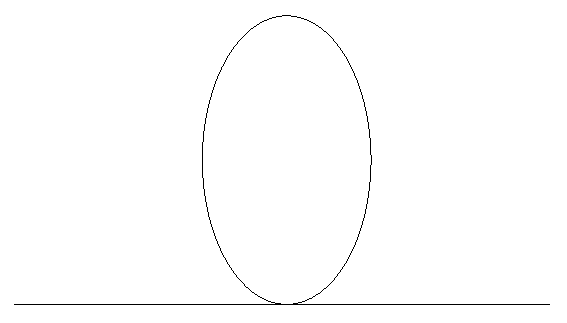
\epsfig{file=lec2-page6-1.eps,width=.3\linewidth}
 
 
\end{center}
 

 
and all those which contain such a loop-like graph as a subgraph. 
Indeed, these graphs produce a constant function of $k^2$,
so they can be removed by renormalization of mass.
More precisely, there exists a function $P(\L,g)=gP_1(\L)+g^2P_2(\L)+...$, 
such that 
the sum of terms corresponding to all graphs for the theory 
with mass $m^2$, computed with the cutoff propagator
(see lecture 1) equals the sum of terms corresponding only to graphs
without loop-like subgraphs, but with mass $M(\L)$ such that 
$M^2=m^2+P(\L,g)$. So we can assume from the beginning that 
we have a theory with mass $M(\L)$ and not worry about loop-like graphs. 

Now we have no divergent graphs with one internal vertex, so
we have no corrections to make in the first order in $g$. 
Let us look at the second order in $g$. 
In this case we have the following bad graphs: 

\begin{center} 
 
\epsfig{file=lec2-page6-2.eps,width=.8\linewidth}
 
\end{center}

Denote the first graph by $\Gamma_2$ and the second by $\Gamma_4$. 

Thus, in order $g^2$ we have a problem in the 2-point and the 4-point 
functions. The problem in the 2-point function is
created by $\Gamma_2$. The graph $\Gamma_2$ diverges quadratically. 
Therefore, 
the term corresponding to $\Gamma_2$ 
computed using the cutoff propagator is a 
function of $k^2,\L$ of the form
$g^2\Sigma_2(k^2,\L)$, where 
$$
\Sigma_2(k^2,\L)=Ak^2\ln(\L/\mu)+B(\L)+
O(1), B(\L)=B_0\L^2(1+o(1)),\L\to +\infty
\leqno{(2.15)}
$$
This asymptotics follows from the fact that the first derivative of
(2.15) with respect to
$k^2$ is logarithmically divergent, and the second one is convergent.

Another problem we have is in the 4-point function, created by the graph
$\Gamma_4$. 
This graph is logarithmically divergent. 
This means, if we compute
the term corresponding to this graph using the cutoff propagator,
we will get a function of $k_i,\L$ of the form
$g^2\Theta_2(k_1,k_2,k_3,\L)$, where 
$$
\Theta_2(k_1,k_2,k_3,\L)=C\ln(\L/\mu)+
O(1),\L\to +\infty
\leqno{(2.16)}
$$
This asymptotics follows the fact that the derivative of the integral
corresponding to $\Gamma_4$ with respect to $k_i$ is convergent.
 
In order to renormalize the 2- and 4- point functions in order $g^2$, we
choose renormalized functions $\Sigma_2^R(k^2)$,
$\Theta_2^R(k_1,k_2,k_3)$. Here $\Sigma_2^R$ is an arbitrary
function of $k^2$ whose second derivative is given by the 
(convergent!) integral obtained by applying 
$\biggl(\frac{d}{dk^2}\biggr)^2$ to the quadratically divergent
integral corresponding to $\Gamma_2$. Analogously,
$\Theta_2^R$ is an arbitrary
function of $k_1,k_2,k_3$ whose derivatives are given by the 
convergent integrals obtained by differentiating
 the logarithmically divergent
integral corresponding to $\Gamma_4$.
 It is clear that the function
$\Sigma_2^R$ is defined uniquely up to addition of a 
function of $k^2$ of the form $ak^2+b$, and the function $\Theta_2^R$ is
defined uniquely up to addition of a constant. 
  
Now we will make second order corrections 
to the coefficients of $(\nabla\phi)^2$, $\phi^2$ and $\phi^4$
in the Lagrangian. 
Namely, we will consider a new Lagrangian of the form
$$
{\cal L}=\int \biggl(\frac{1}{2}(\nabla\phi)^2+
\frac{M^2}{2}\phi^2
+\frac{g}{4!}\phi^4+\frac{\alpha(\L)}{2}(\nabla\phi)^2+
\frac{\beta(\L)}{2}\phi^2+\frac{\gamma(\L)}{4!}\phi^4\biggr)d^nx,
\leqno{(2.17)}
$$
Let $\Sigma_2'(k^2,\L,\alpha,\beta,\gamma)$,
$\Theta_2'(k_1,k_2,k_3,\L,\alpha,\beta,\gamma)$ be the functions 
$\Sigma_2$, $\Theta_2$ 
for this Lagrangian and the cutoff propagator. 
We will choose the functions $\alpha,\beta,\gamma$ in such a way
that 
$$
\begin{aligned}
\lim_{\L\to\infty}\Sigma_2'(k^2,\L,m,\alpha(\L),\beta(\L),\gamma(\L))&=
\Sigma_2^R(k^2),\\
\lim_{\L\to\infty}\Theta_2'(k_1,k_2,k_3,\L,m,\alpha(\L),\beta(\L),\gamma(\L))&=
\Theta_2^R(k_1,k_2,k_3),\\
\end{aligned}
\leqno{(2.18)}
$$
As we are working modulo $g^3$, we can choose 
$\alpha,\beta,\gamma$ in the form
$\alpha=g^2\alpha_2$, $\beta=g^2\beta_2$, 
$\gamma=g^2\gamma_2$, where 
$\alpha_2,\beta_2,\gamma_2$ are independent of $g$. It is easy to check
that in order for (2.18) to hold, the functions
 $\alpha_2,\beta_2,\gamma_2$ 
should have the following asymptotics:
$$
\begin{aligned}
\alpha_2=g^2(A\ln(\L/m)+D_1)+o(1), \beta_2&=
g^2(-B(\L)+D_2)+o(1),\\
\gamma_2&=g^2(C\ln(\L/m)+D)+o(1),\L\to+\infty,
\end{aligned}
\leqno{(2.19)}
$$
where $D_1,D_2$ depend on the choice of $\Sigma_2^R$, and
$D$ depends on the choice of $\Theta_2^R$.
Of course, there are many ways to choose such functions, but
they are unique up to adding terms $o(1)$, $\L\to\infty$.

Thus, we have renormalized the graphs $\Gamma_2$, $\Gamma_4$.
This removes 
divergence in all correlation functions modulo $g^3$.
Thus, all correlation functions of our theory are now defined 
modulo $g^3$. 

Now we proceed inductively in the order of $g$. Suppose we have 
removed divergences and defined all correlation functions modulo $g^K$. 
Consider the $2N$-point function 
(for the deformed Lagrangian and the cutoff propagator) modulo $g^{K+1}$:
$$
F_{2N}=\sum_{j=0}^{K-1}g^jF_{2N,j}^R+g^KF_{2N,K}\leqno{(2.20)}
$$
(the superscript $R$ means that the corresponding coefficient
has already been renormalized).
The term $F_{2N,K}$ is represented by the sum over all graphs with 
$K$ internal vertices. This sum has superficial divergence index
$4-2N$. Therefore, the second derivative of $F_2$ by $k^2$, 
the first partial derivatives of $F_4$, and $F_{2N}$, $N\ge 3$, are 
superficially convergent. The crucial fact for renormalization theory, 
which follows from the ``Strong Weinberg Theorem'' (see Lecture 1), is

\proclaim{Proposition 2.2} There exists finite limits, as $\L\to\infty$, of
the functions $F_{2N,K}(k_1,...,k_{2N-1},\L)$,
$\nabla_kF_{4,K}(k_1,k_2,k_3,\L)$, 
and $\biggl(\frac{d}{dk^2}\biggr)^2F_{2,K}(k^2,\L)$
$N\ge 3$. 
\endproclaim

{\bf Remark.} For $\phi^4$ theory, this proposition holds for 
the term corresponding to each particular graph, but in general
(for example, for theories with gauge fields) this is not the case:
the sum over all graphs may have a meaning while each individual
graph does not. However, an analogue of Proposition 2.2 
(for the sum over all graphs) holds in any renormalizable theory. 

Proposition 2.2 allows us to fulfil the induction step. It shows that
the function $F_2$ (in the limit) is defined up to adding $ak^2+b$, 
the function $F_4$ is defined up to adding a constant, and $F_{2N}$, $N\ge
3$, is defined uniquely. So one can choose renormalized functions
$F_{2N,K}^R$ and make corrections in the Lagrangian,
$\alpha\to\alpha+g^K\alpha_K$, $\beta\to\beta+g^K\beta_K$,
$\gamma\to\gamma+g^K\gamma_K$, to compensate the divergence in $F_{2N,K}$ 
and obtain $F_{2N,K}^R$ instead of it. This procedure is completely
analogous to the one for order $g^2$. In this way we will complete 
the renormalization in order $K$.

{\bf Remark 1.} At every step of our renormalization procedure we 
had to choose 3 constants of integration. This may create an impression
that we get a family of theories parametrized by 3 infinite sequences 
of constants. However, it is easy to see
that in fact we get a family of theories parametrized 
by only 3 constants. This means that any 4 invariants attached to 
the theory (for example, values of the 2-point function at 4 points in 
spacetime) are linked by a universal  
functional relation. 
 
{\bf Remark 2.} Even if in the original theory certain critical
or subcritical interactions were not present, they may appear 
in the process of renormalization. 
In general,
renormalization brings in all missing critical and subcritical
terms, unless there is a symmetry which prevents it from doing so.
Let us demonstrate it by a few examples. 

{\bf Example 1.} 
In the process of 
renormalization of the Lagrangian (2.12) in 4 dimensions we will be forced to 
introduce the subcritical term $\phi^3$ and the critical term
$\phi^4$, in order 
to remove logarithmic divergence in the graphs 
\begin{center} 
 
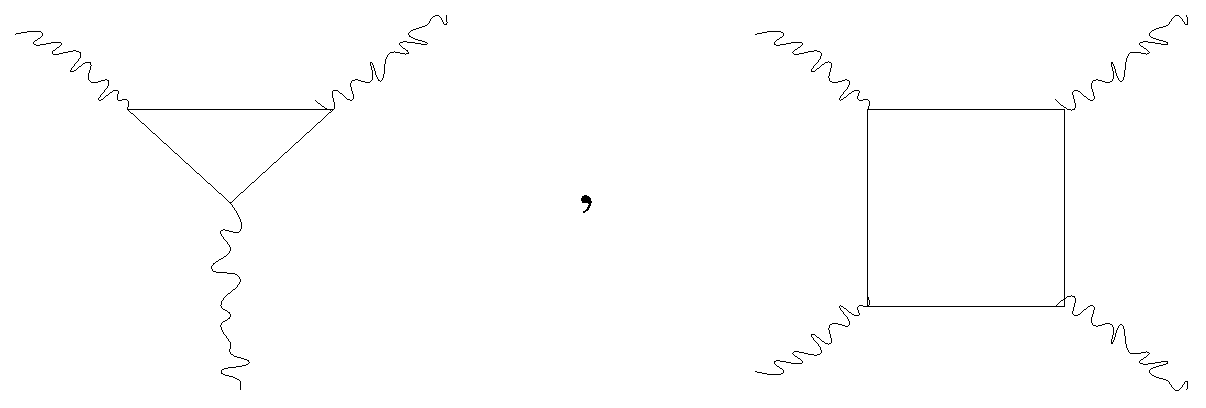
\epsfig{file=lec2-page9-1.eps,width=.8\linewidth}
 
\end{center}



where wavy lines correspond to bosons and straight ones to fermions. 
However, the critical term $\phi^2\nabla\phi$ will not appear, since there
is no Poincare invariant expression of this form. In terms of graphs, this
means that the graph

\begin{center} 
 
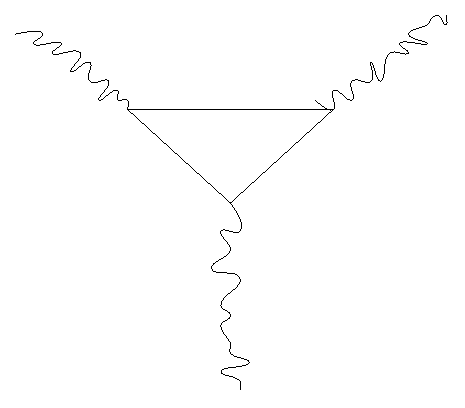
\epsfig{file=lec2-page9-2.eps,width=.3\linewidth}
 
 
\end{center}


whose superficial divergence is linear, in fact diverges
only logarithmically, because of cancellations in the integrand 
caused by Poincare symmetry; so there is no linear divergence to compensate
and hence no need for $\phi^2\nabla\phi$ to appear.  

{\bf Example 2.} In $\phi^4$ theory in 4 dimensions, the subcritical 
term $\phi^3$ does not appear in renormalization, since it is not preserved
by the symmetry $\phi\to -\phi$ of the original theory.
In the language of graphs, this is clear: there is no graphs 
with 3 external edges, so there is no divergence to compensate
by $\phi^3$.

 In a general field theory, 
every type (in terms of external edges) 
of a superficially divergent graph corresponds to a 
number of critical and subcritical 
terms in the Lagrangian, which should be renormalized
in order compensate the divergence in the corresponding graph. 
More precisely, divergent terms which are quadratic 
in $k$ correspond to terms in the Lagrangian which have two 
derivatives by $x$, linear terms in $k$ 
correspond to terms with one derivative, and constant 
divergencies correspond to terms without derivative. 

{\bf Remark.} It follows from formula (2.4) that
in a renormalizable theory, all divergences in $N\ge 2$-point 
correlation function are no worse than quadratic.
So the coefficient of $k^2$ in the 2-point function
if divergent at most logarithmically. 
Therefore, if the quadratic forms $Q_i$ have to be renormalized
(like in $\phi^4$ theory), 
they will be multiplied by coefficients which depend 
on the cutoff parameter $\L$ at worst logarithmically. This shows that
the dimension of $Q_i$ and hence of $\phi_i$ survives renormalization
to all finite orders in the asymptotic expansion.



\end{document}
  


